%!TEX root = CooperBarba2014.tex

To obtain the following results, we extended the \pygbe code to consider surfaces with prescribed charge or potential. For most runs, we used a workstation with Intel Xeon X5650 \cpu s  and one \nvidia Tesla C2075 \gpu\ card (2011 Fermi). That includes the code verification runs using the analytical solution and the calculations with protein G B1 D4$^\prime$. The final case considers the antibody immunoglobulin G, which is a much larger molecule than protein G. For these runs, we used Boston University's \textsc{bungee} cluster, which has 16 nodes with 8 Intel Xeon \cpu\ cores each, and a total of 3 \nvidia Tesla Kepler K20 and 26 \nvidia Tesla M2070/2075 \gpu s. All runs were serial: single-\cpu\ and single-\gpu. We used the free \msms software\cite{SannerOlsonSpehner1995} to generate meshes, and \texttt{pdb2pqr}\cite{Dolinsky04} with an \amber forcefield to determine the charges and van der Waals radii. In these tests, we did not consider a Stern layer for either the protein or the charged surface, nor the presence of solvent-filled cavities inside the protein.

\subsection{Verification against analytical solution} \label{sec:verification}

Using the analytical solution detailed in Section \ref{sec:analytical_solution}, we carried out a grid-convergence study of \pygbe extended to treat interacting surfaces with biomolecules. The setup consists of a spherical molecule with a $5$\AA~radius and a centered charge of $1e^-$, interacting with a spherical surface of $4$\AA~radius and an imposed potential of $\phi=1$. The center-to-center distance between the spheres is $12$\AA, and they are dissolved in water with salt at 145mM, which gives a Debye length of 8 ($\kappa = 0.125$), and permittivity $\epsilon_\text{sol} = 80$. The permittivity inside the spherical protein is $\epsilon_\text{mol} = 4$. Figure \ref{fig:twosphere_num} shows a sketch of this system.

\begin{figure}[h] %  figure placement: here, top, bottom, or page
   \centering
   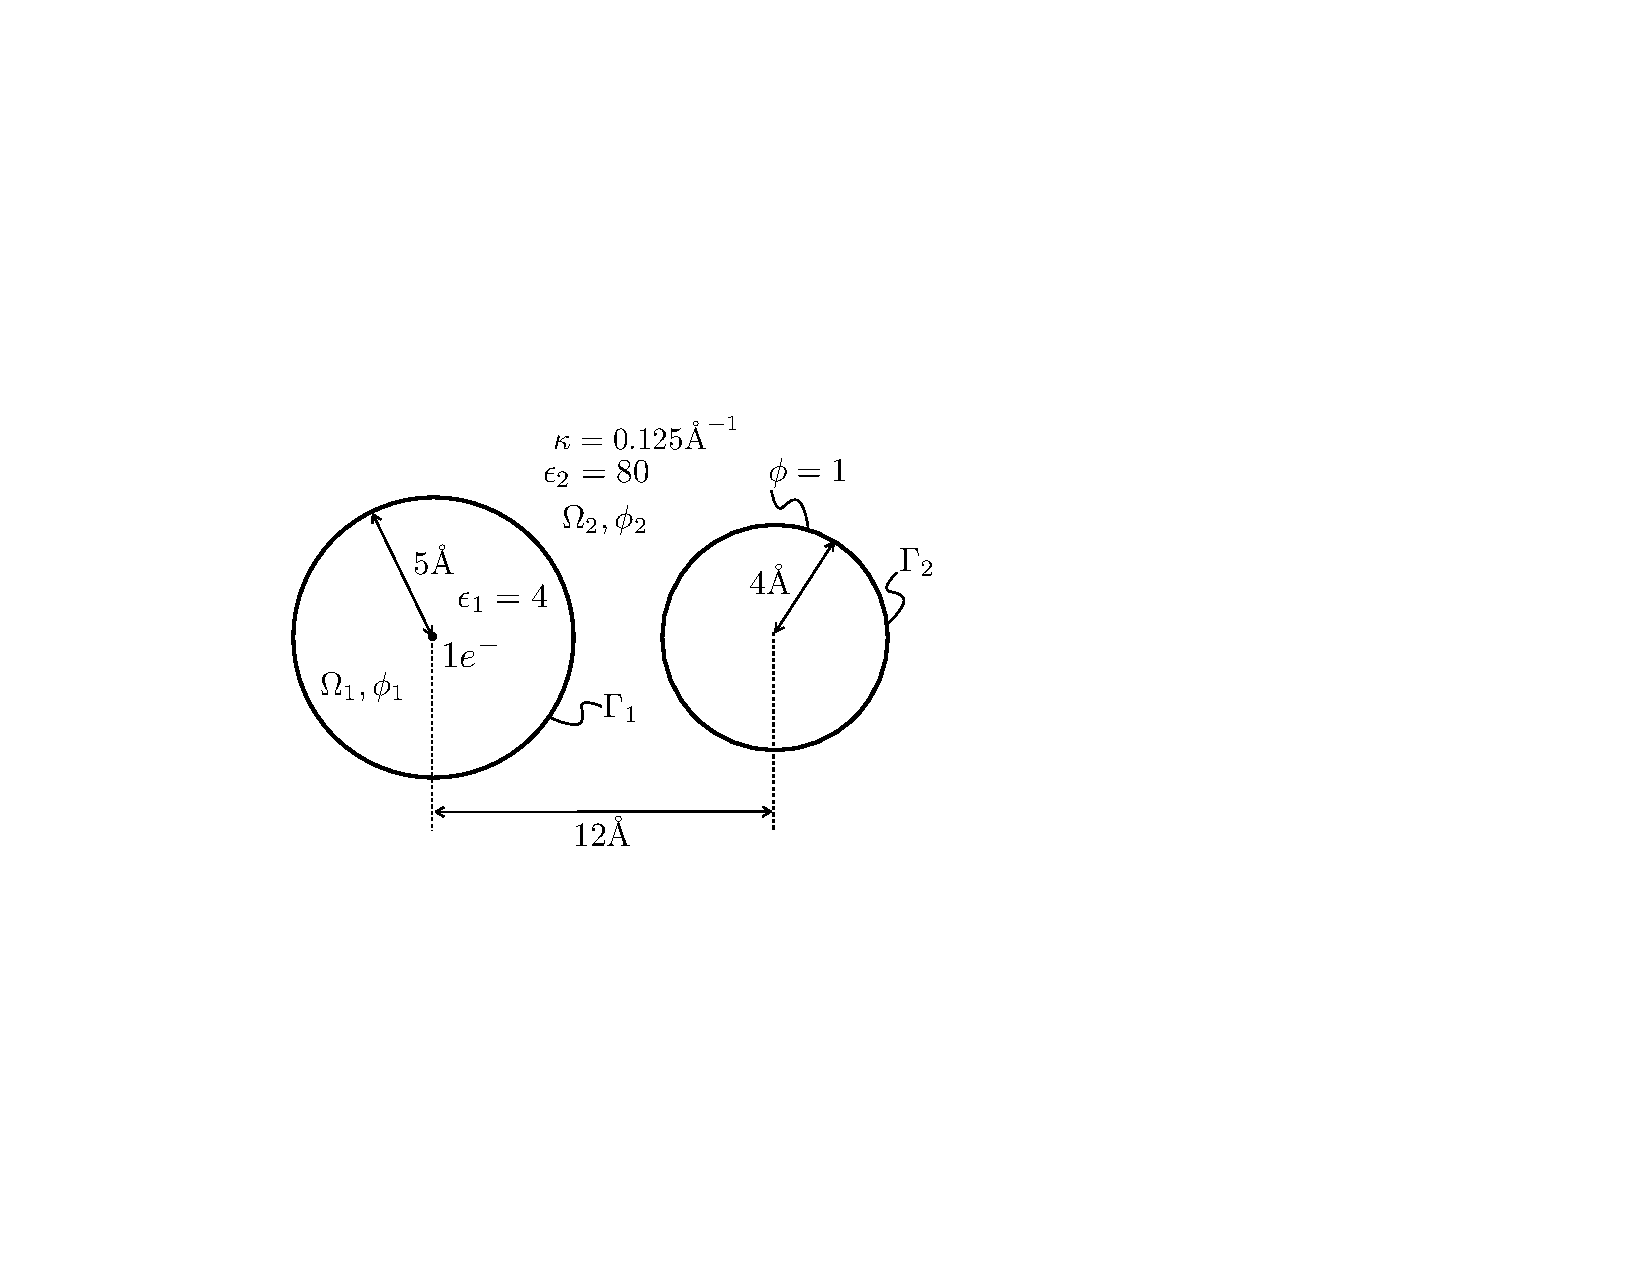
\includegraphics[width=0.45\textwidth]{Figure8.pdf} 
   \caption{Sketch of system used in the convergence study of Figure \ref{fig:error_sphere}.}
   \label{fig:twosphere_num}
\end{figure}

Figure \ref{fig:error_sphere} presents the results of the grid-convergence analysis, where the error is the relative difference in interaction free energy between the analytical result from Section \ref{sec:analytical_solution} and the numerical solution computed with \pygbe. The observed order of convergence of the three finest meshes was 1.007. Table \ref{table:params1} presents the numerical parameters used in this case. Recall from section \ref{sec:methods} that we calculate the boundary-element integrals differently for close-by and far-away elements, and use a semi-analytical method for the element that contains the collocation point. The fine Gauss quadrature rule is used for elements closer than $2L$ from the collocation point, where $L=\sqrt{2\cdot \text{Area}}$. For the treecode,  $N_{\text{crit}}$ is the maximum number of boundary elements per box, $P$ is the Taylor expansion truncation parameter and $\theta$ is the multipole-acceptance criterion. The final numerical parameter is the exit tolerance of the \textsc{gmres} solver.

\begin{table}[h]
  %\centering
   %\fontfamily{ppl}\selectfont
   \caption{\label{table:params1}Numerical parameters used in the code-verification runs with the analytical solution. } 
    \begin{tabular}{c c c c c c c}
	\hline%\toprule
	\multicolumn{3}{l} {\# Gauss points:} & \multicolumn{3}{l}{Treecode:} & \gmres:\\
	\footnotesize{in-element} & \footnotesize{close-by} & \footnotesize{far-away} & $N_{\text{crit}}$ & $P$ &  $\theta$  & tol.\\
	\hline%\midrule
	9 per side & 37 & 3  &  300 & 15 & 0.5  & $10^{-9}$\\	
	\hline%\bottomrule
    \end{tabular}
\end{table}


\begin{figure}[htbp] %  figure placement: here, top, bottom, or page
   \centering
   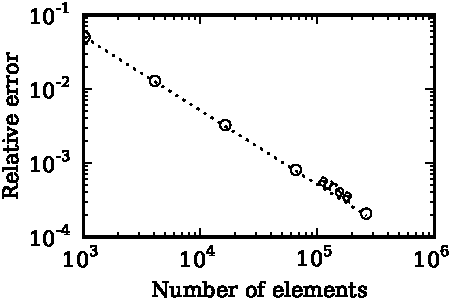
\includegraphics[width=0.4\textwidth]{Figure9.pdf} 
   \caption{Grid-convergence study for the interaction free energy between a spherical molecule with a centered charge and a sphere with potential $\phi=1$. Data sets, figure files plus running/plotting scripts are available under \ccby.\cite{CooperBarba2015-share1348841}}
   \label{fig:error_sphere}
\end{figure}

As seen in Figure \ref{fig:error_sphere}, the error decays with the average area of the boundary elements ($\frac{1}{N}$), which is the expected behavior considering our previous work. \cite{CooperBarba-share154331} This proves that the extension of \pygbe to treat charged surfaces is solving the mathematical model correctly.

%The interaction free energy involves three separate calculations: one with both bodies (molecule and interacting surface with set potential) and one for each isolated body. The time to solution for each mesh in Figure \ref{fig:time} corresponds to the total time, including all three cases that need to be computed. The most time consuming part of the algorithm is the matrix-vector product within the Krylov solver, which scales as $O(N \log N)$ thanks to the treecode acceleration. However, the total time to solution scales slightly worse than $O(N \log N)$. This happens because the condition number of the system depends on the number of elements and more iterations are required to converge to the specified tolerance, which is revealed by Figure \ref{fig:iterations}.

\subsection{First case: protein G B1 D4$^{\prime}$} \label{sec:PGB}

We computed the electrostatic field of protein G B1 D4$^{\prime}$ interacting with a 100\AA$\times$100\AA$\times$10\AA\ block with surface charge density $\pm$0.05C/m$^2$, and investigated its preferred orientation. The protein was centered with respect to a  100\AA$\times$100\AA\ face, a distance 2\AA\ above it. 
As seen in Figure \ref{fig:1pgb_orientation}, $\alpha_\text{tilt}$ is the angle between the protein's dipole moment and the normal vector to the surface, and $\alpha_\text{rot}$ rotates about the dipole moment. The dipole-moment vector placed at the center of mass of the protein generates an axis, and we used the line of shortest distance between the outermost atom and this axis as a reference vector $\mathbf{V}_{\text{ref}}$. The rotation angle $\alpha_{\text{rot}}$ is the angle between the normal vector to a 100\AA$\times$10\AA\ side face of the block and $\mathbf{V}_{\text{ref}}$.

In these cases, we considered a solvent with no salt, i.e., $\kappa=0$ (to compare with other published results), and with relative permittivity 80. The region inside the protein had a relative permittivity of 4.

\medskip

 \paragraph*{Grid-convergence study for protein G B1 D4$^{\prime}$---}

By means of a grid-convergence study, we make sure that the runs are in the asymptotic range of the model, select a triangle density so that the geometry is well-resolved by the surface mesh, and find adequate values of the simulation parameters for sampling the orientations. Using Richardson extrapolation, we find values of the energy that estimate the exact solution and use them as a reference to calculate estimated errors. This error is simply the relative difference between the energy obtained numerically with each mesh density and the estimated exact value. In this way, we choose the parameters for the sampling runs with confidence that they are both accurate and efficient in computing time. 

We computed the solvation and surface energy of a system containing a surface with charge density 0.05C/m$^2$, and a protein at $\alpha_{\text{tilt}} = 10^{\circ}$ and $\alpha_{\text{rot}} = 200^{\circ}$. The numerical parameters are presented in Table \ref{table:params2}. Using runs with mesh densities of 2, 4, and 8 elements per square Angstrom, we obtained the values in Table \ref{table:extraPGB} using Richardson extrapolation: these are the reference values for the error plotted in Figure \ref{fig:convergence_1PGB_sensor}. The observed order of convergence was 0.96 for the solvation energy and 0.94 for the surface energy. For details on the Richardson-extrapolation method for performing grid-convergence analysis, see our previous work.\cite{CooperBardhanBarba2013} 
Figure \ref{fig:convergence_1PGB_sensor} shows errors that are decaying as $1/N$ in both the solvation and surface energies for the finest three meshes. This indicates that the calculations are in the asymptotic region and the geometry is well resolved in these cases.

\begin{table}[h]
  %\centering
   %\fontfamily{ppl}\selectfont
   \caption{\label{table:params2}Numerical parameters used in the convergence runs with protein G B1 D4$^{\prime}$. } 
    \begin{tabular}{c c c c c c c}
	\hline%\toprule
	\multicolumn{3}{l} {\# Gauss points:} & \multicolumn{3}{l}{Treecode:} & \gmres:\\
	\footnotesize{in-element} & \footnotesize{close-by} & \footnotesize{far-away} & $N_{\text{crit}}$ & $P$ &  $\theta$  & tol.\\
	\hline%\midrule
	9 per side & 19 & 7  &  500 & 15 & 0.5  & $10^{-8}$\\	
	\hline%\bottomrule
    \end{tabular}
\end{table}



\begin{table}[h]
  %\centering
   %\fontfamily{ppl}\selectfont
   \caption{\label{table:extraPGB}Extrapolated values of energy for protein G B1 D4$^\prime$.} 
    \begin{tabular}{c c}
	\hline%\toprule
	\multicolumn{2}{c} {Energy [kcal/mol]} \\
	Solvation & Surface \\
	\hline%\midrule
	$-222.43$ & $317.98$ \\	
	\hline%\bottomrule
    \end{tabular}
\end{table}

\begin{figure}[h] %  figure placement: here, top, bottom, or page
   \centering
   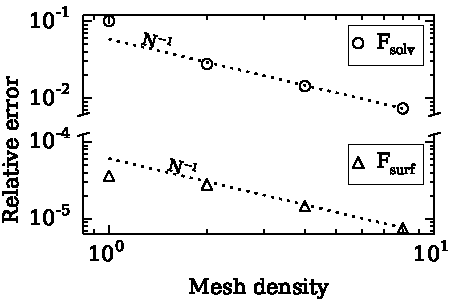
\includegraphics[width=0.45\textwidth]{Figure10.pdf} 
   \caption{Grid-convergence study of the solvation and surface energy for protein G B1 D4$^{\prime}$ mutant, interacting with a surface with a charge density of 0.05C/m$^2$. Data sets, figure files and running/plotting scripts available under \ccby.\cite{CooperBarba2015-share1348803}}
   \label{fig:convergence_1PGB_sensor}
\end{figure}



%%% COMMENTED OUT SECTION
\begin{comment}
\begin{figure*}
   \centering
   \subfloat[]{\includegraphics[width=0.45\textwidth]{1IGT_cos.pdf} \label{fig:1IGT_cos}}
   \subfloat[]{\includegraphics[width=0.45\textwidth]{1IGT_alpha.pdf} \label{fig:1IGT_alpha}}\\
   \subfloat[]{\includegraphics[width=0.45\textwidth]{1IGT_2D_sig005.pdf} \label{fig:1IGT_2D_sig005}}
   \subfloat[]{\includegraphics[width=0.45\textwidth]{1IGT_2D_sig-005.pdf} \label{fig:1IGT_2D_sig-005}}
   \caption{Orientation distribution of immunoglobulin G. Figures \ref{fig:1IGT_cos} and \ref{fig:1IGT_alpha} are the probability with respect to the tilt angle and its cosine, respectively. Figures \ref{fig:1IGT_2D_sig005} and \ref{fig:1IGT_2D_sig-005} are the orientation with respect to both the tilt and rotation angle.}
   \label{fig:1IGT_probability}
\end{figure*}

\begin{figure*}
   \centering
   \subfloat[Side view for $\alpha_{\text{tilt}} = 116^{\circ}$ and $\alpha_{\text{rot}} = 100^{\circ}$]{\includegraphics[width=0.45\textwidth]{1IGT_3D_sig-005_til116_rot100_side.pdf} \label{fig:1IGT_sig-005_side}}
   \subfloat[Top view for $\alpha_{\text{tilt}} = 116^{\circ}$ and $\alpha_{\text{rot}} = 100^{\circ}$]{\includegraphics[width=0.45\textwidth]{1IGT_3D_sig-005_til116_rot100_top.pdf} \label{fig:1IGT_sig-005_top}}\\
   \subfloat[Side view for $\alpha_{\text{tilt}} = 64^{\circ}$ and $\alpha_{\text{rot}} = 280^{\circ}$]{\includegraphics[width=0.45\textwidth]{1IGT_3D_sig005_til064_rot280_side.pdf} \label{fig:1IGT_sig005_side}}
   \subfloat[Top view for $\alpha_{\text{tilt}} = 64^{\circ}$ and $\alpha_{\text{rot}} = 280^{\circ}$]{\includegraphics[width=0.45\textwidth]{1IGT_3D_sig005_til064_rot280_top.pdf} \label{fig:1IGT_sig005_top}}
   \caption{Surface potential for Immunoglobulin G for the preferred orientation according to Figure  \ref{fig:1IGT_probability} for $\sigma$=-0.05 C/m$^2$ in Figures \ref{fig:1IGT_sig-005_side} and \ref{fig:1IGT_sig-005_top} and $\sigma$=0.05 C/m$^2$ in Figures \ref{fig:1IGT_sig005_side} and \ref{fig:1IGT_sig005_top}. The black arrow indicates the direction of the dipole moment.}
   \label{fig:1IGT_3D}
\end{figure*}
\end{comment}
%%% END COMMENT


%%% COMMENTED OUT SECTION
\begin{comment} 

\subsection{Fc-protein G complex} \label{sec:FCC}

We simulated the electrostatic field of the complex generated by the Fc fragment of immunoglobulin G and protein G B1 interacting with a $250\times10\times250$\AA \xspace block with surface charge density $\pm$0.05C/m$^2$, to find its preferred orientation. The protein was centered with respect to a  $250\times250$\AA \xspace face, 5\AA \xspace above it, and the orientation was defined by $\alpha_{\text{tilt}}$ and $\alpha_{\text{rot}}$, like in Section \ref{sec:PGB}. 

In these cases, we considered a 0.150M of salt in the solvent, i.e. $\kappa=0.125$, with relative permittivity 80. The region inside the protein had a relative permittivity of 4.

 \paragraph*{Mesh refinement study for Fc-protein G complex}

Similar to Section \ref{sec:PGB}, we performed a mesh refinement study to make sure the geometry was well resolved and to find appropriate simulation parameters for sampling different orientations. 

In these runs, we evaluated the solvation energy and surface energy of a system with a surface with charge density 0.05C/m$^2$, and a protein with $\alpha_{\text{tilt}} = 100^{\circ}$ and $\alpha_{\text{rot}} = 45^{\circ}$. Using the results from runs with mesh density 2, 4, and 8 elements per square Angstrom, we added the solvation and surface energies, and extrapolated them using Richardson extrapolation to obtain -1390.59 kcal/mol, with observed order of convergence 1.1. This value is the reference to calculate the errors in Figure \ref{fig:1FCC_convergence}. 

For the mesh refinement study, we used 1 Gauss points per far-away element, 19 Gauss points per close-by element, and 9 Gauss points per triangle side for the singular integral. The treecode had 6 terms in the Taylor expansion, a multipole-acceptance criterion of 0.5, and no more than 1000 boundary elements per box of the lowest level of the tree. Also, the GMRES tolerance was 10$^{-4}$. 

\begin{figure}[h] %  figure placement: here, top, bottom, or page
   \centering
   \includegraphics[width=0.5\textwidth]{1FCC_convergence.pdf} 
   \caption{Mesh convergence study of the solvation plus surface energy for the Fc-protein G complex interacting with a surface with charge density 0.05C/m$^2$.}
   \label{fig:1FCC_convergence}
\end{figure}

Figure \ref{fig:1FCC_convergence} show errors that are decaying as $1/N$ for both the solvation and surface energies, indicating that the geometry is well resolved.

 \paragraph*{Probing orientation of Fc-protein G complex}

We sampled the total free energy every $\Delta \alpha_{\text{tilt}} = 2^\circ$ of tilt angle and $\Delta \alpha_{\text{rot}} =20^\circ$ of rotation angle.  In these runs, meshes had 2 triangles per square angstrom throughout. We used 1 Gauss point per element further away than 2L of the collocation point, 19 Gauss points for close-by elements, and 9 Gauss points per side of the singular element. The treecode used 2 terms in the Taylor expansion, a multipole-acceptance criterion of 0.5 and no more than 300 elements per lowest level box. The GMRES tolerance was 10$^{-4}$. 

The total free energy was the input for numerically computing the integrals in Equation \eqref{eq:prob_angle} with the trapezoidal rule. Figure \ref{fig:probability} shows the probability of the protein orientation in terms of $\cos(\alpha_{\text{tilt}})$, in intervals of $\Delta \cos(\alpha_{\text{tilt}}) = 0.05$ for Figure \ref{fig:1FCC_cos}, and $\Delta \alpha_{\text{tilt}}$=4$^{\circ}$ for Figure \ref{fig:1IGT_alpha}.  

\begin{figure*}
   \centering
   \subfloat[]{\includegraphics[width=0.45\textwidth]{1FCC_cos.pdf} \label{fig:1FCC_cos}}
   \subfloat[]{\includegraphics[width=0.45\textwidth]{1FCC_alpha.pdf} \label{fig:1FCC_alpha}}\\
   \subfloat[]{\includegraphics[width=0.45\textwidth]{1FCC_2D_sig005.pdf} \label{fig:1FCC_2D_sig005}}
   \subfloat[]{\includegraphics[width=0.45\textwidth]{1FCC_2D_sig-005.pdf} \label{fig:1FCC_2D_sig-005}}
   \caption{Orientation distribution of Fc-protein G complex. Figures \ref{fig:1FCC_cos} and \ref{fig:1FCC_alpha} are the probability with respect to the tilt angle and its cosine, respectively. Figures \ref{fig:1FCC_2D_sig005} and \ref{fig:1FCC_2D_sig-005} are the orientation with respect to both the tilt and rotation angle.}
   \label{fig:1FCC_probability}
\end{figure*}

\begin{figure*}
   \centering
      \subfloat[Side view for $\alpha_{\text{tilt}} = 20^{\circ}$ and $\alpha_{\text{rot}} = 160^{\circ}$]{\includegraphics[width=0.49\textwidth]{1FCC_sig005.pdf}\label{fig:1FCC_sig005}} 
   \subfloat[Side view for $\alpha_{\text{tilt}} = 120^{\circ}$ and $\alpha_{\text{rot}} = 20^{\circ}$]{\includegraphics[width=0.49\textwidth]{1FCC_sig-005.pdf} \label{fig:1FCC_sig-005}}
   \caption{Surface potential for Fc-protein G complex in the preferred orientation according to Figure \ref{fig:1FCC_probability} for $\sigma$=0.05 C/m$^2$ in Figure \ref{fig:1FCC_sig005}, and $\sigma$=-0.05 C/m$^2$ in Figure \ref{fig:1FCC_sig-005}. The black arrow indicates the direction of the dipole moment.}
   \label{fig:1IGT_3D}
\end{figure*}

%%% END COMMENT OUT
\end{comment} 
